%%%%%%%%%%%%%%%%%%%%%%%%%%%%%%%%%%%%%%%%%%
% Master Thesis 
% Polina Polunina
% October 2022 
%
% License:
% CC-BY-SA 4.0 -- Creative Commons Attribution-ShareAlike 4.0 International
% https://creativecommons.org/licenses/by-sa/4.0/legalcode
%%%%%%%%%%%%%%%%%%%%%%%%%%%%%%%%%%%%%%%%%%
\section{State-of-the-art}

From the beginning of the COVID-19 pandemic, several approaches have been presented to determine SARS-CoV-2 in wastewater samples. In \autoref{sec:prior:methods}, I will give an overview of existing tools and pipelines. In this section, I consider some tools and pipelines aiming to detect SARS-CoV-2 lineages and their abundance in wastewater samples. This determination can be focused on \acrfull{vocs} as well as \acrfull{vois} and additionally with an intention to detect newly appeared unknown variants. In \autoref{sec:prior:discussion}, I will give a short discussion of the existing methods with respect to the goals of this thesis.

    \subsection{Methods for wastewater surveillance} \label{sec:prior:methods}
    
    To list the existing tools/pipelines representing such approaches, \cref{tab:prior:methods} shows some of them accompanied by a link to the source code and a description of produced outputs.
        
        \begin{table}[ht!]
            \centering
            \small
            \begin{tblr}{l|ll}
             \textbf{Name}          & \textbf{Output} \\     \hline 
            \textbf{Freyja}         & a TSV file that includes the lineages present, their corresponding\\
                                    & abundances, and summarization by constellation.\\
                                    & Additional option: a fast bootstrapping method for Freyja which\\
                                    & results in two output files base-name-lineages.csv and\\
                                    & base-name\_summarized.csv, which contain the 0.025, 0.05,0.25,0.5\\
                                    & (median),0.75, 0.95, and 0.975 percentiles for each lineage and\\
                                    & WHO designated VOI/VOC, respectively, as obtained via the bootstrap.\\
                                    & They also provide the --eps, --barcodes, and --meta options as in\\
                                    & Freyja demix. We now also provide a --boxplot option, which should\\
                                    & be specified in the form --boxplot pdf if you want the boxplot in\\
                                    & pdf format.\\ \hline[dashed]
            \textbf{COJAC}          & - total count of amplicons carrying the sites of interest;\\
                                    & - amplicons carrying mutations on all sites of interest (e.g.: variant\\
                                    & mutations observed on all sites);\\
                                    & - amplicons where one mutation is missing (e.g.: only 2 out of 3 sites\\
                                    & carried the variant mutation, 1 site carries wild-type);\\
                                    & - fraction (ratio of number of all amplicons carrying mutations on all\\
                                    & sites of interest to the total number of amplicons carrying cites of\\
                                    & interest) or empty if no counts;\\
                                    & - number of a considered sites (e.g.: 2 sites of interests) or empty if\\
                                    & no counts.\\  \hline[dashed]
            \textbf{LCS}            &- lineage deComposition outputs for SARS-CoV-2 pooled samples\\
                                    & - plots file of python format \\ \hline[dashed]
            \textbf{Kallisto}       & -abundance.h5 is an HDF5 binary file containing run info, abundance\\
                                    & estimates, bootstrap estimates, and transcript length\\
                                    & information length. This file can be read by sleuth\\
                                    & -abundance.tsv is a plaintext file of the abundance estimates. It\\
                                    & does not contain bootstrap estimates. Please use the --plaintext mode\\
                                    & to output plaintext abundance estimates. Alternatively, Kallisto h5dump\\
                                    & can be used to output an HDF5 file to plaintext. The first line\\
                                    & contains a header for each column, including estimated counts, TPM,\\
                                    & and effective length.\\
                                    & -run\_info.json is a JSON file containing information about the run\\  \hline[dashed]
            \textbf{Alcov}          & - the number of reads with and without each mutation in each sample;\\
                                    & - heatmap showing the frequencies for all samples;\\
                                    & - mutations.txt;\\
                                    & - read depth for each amplicon;\\
                                    & - Plotting amplicon GC content against amplicon depth\\  \hline[dashed]
            \end{tblr}
         \end{table}
         \begin{table}[ht!]
            \centering
            \small
            \begin{tblr}{l|ll}
             \textbf{Name}          & \textbf{Output} \\     \hline 
            \textbf{Pipes et al.}   & - estimated proportion of candidate strains in .csv file\\
                                    & - barplot in the .pdf file. Only those strains with an estimated\\
                                    & proportion larger than 1\% will appear in this plot;\\
                                    & - for unidentifiable strains, groups of unidentifiable strains will\\
                                    & be printed to a .txt file. If there is no identifiability issue,\\
                                    & this .txt file will not be produced.\\  \hline[dashed]
            \textbf{SAM refiner}    & SAM Refiner: SAM Processing produces 4 tab-separated value (TSV) files\\
                                    & that can be read by any standard spreadsheet software;\\
                                    & - SAM Refiner: Chimera Removal produces TSV files - unique sequences;\\
                                    & statistics about removed chimera; covariant deconvolution output;\\
                                    & - XLSX file - assigned sequences to known variant lineages or the\\
                                    & reference based on polymorphisms present. Polymorphisms were\\
                                    & considered for lineage assignment if they appeared in multiple\\
                                    & sequencing runs or were known to be present in circulating populations\\
                                    & reported to GSIAD (https://www.gisaid.org/)\\  \hline[dashed]
            \textbf{Gromstole}      & - counts of each mutation of the lineages;\\
                                    & - coverage at every position on the reference genome;\\
                                    & - metadata;\\
                                    & - estimate of the proportion (including 95\% confidence interval);\\
                                    & - lineage name;\\
                                    & - name of the input directory\\  \hline[dashed]
            \textbf{AG}             & VarScan .tab files (tab-delimited) and common\_depth\_report.csv\\  \hline[dashed]
            \textbf{Lineagespot}    & - VCF, MAF;\\
                                    & - tab-delimited file (TSV file) containing the most probable lineages\\
                                    & that have been found   \\  \hline[dashed]
            \end{tblr}
         \end{table}
         \begin{table}[ht!]
            \centering
            \small
            \begin{tblr}{l|ll}
             \textbf{Name}          & \textbf{Output} \\     \hline 
            \textbf{PiGx}           & -overview report including:\\
                                    & --Visualization of the development of SARS-CoV-2 variants and mutations\\
                                    & over time and locations from all samples provided.\\
                                    & --Quality Control report per sample: number of covered amplicons, read\\
                                    & coverage, and MultiQC report for raw and trimmed reads\\
                                    & --Variants report per sample: variant analysis of SARS-CoV-2 from each\\
                                    & wastewater sample and identification of variants of concern\\
                                    & --Taxonomic classification: a table and pie chart of the species found\\
                                    & in the unaligned reads\\
                                    & -SAM / BAM files per sample: aligned and unaligned reads against\\
                                    & SARS-CoV-2\\
                                    & -VCF / CSV files per sample: listing all detected single nucleotide\\
                                    & variants (SNVs) from the aligned reads\\
                                    & -VEP reports per sample as TXT / HTML: report files show the VEP output\\
                                    & including the uploading variants, including amino acid changes and\\
                                    & consequences for the corresponding protein\\
                                    & -Kraken2 files per sample (txt): provides an overview of all found\\
                                    & species in the unaligned reads together with the NCBI taxonomy ID\\
                                    & -log files for all major analysis steps performed by the pipeline\\  \hline[dashed]
            \textbf{cowwid}         & - co-occurance table;\\
                                    & - variant mutations table;\\
                                    & - plots integrated to CoV-Spectrum.\\  \hline[dashed]
            \textbf{Izquierdo-}     & VCF, MAF files; \\    
            \textbf{Lara et al.}    & - Trees visualisation (Fig tree);\\
                                    & - clades assignment \\  \hline

            \end{tblr}
            \caption{List of existing methods for wastewater surveillance} \label{tab:prior:methods}
        \end{table}
    
        \subsubsection{Freyja}
        One optimized approach for virus concentration from wastewater is proposed by Karthikeyan and co-authors \cite{karthikeyan2022}, they developed and deployed a software that fully resolve multiple virus lineages from wastewater. As a part of the research, they developed a tool called Freyja that detects variants from SARS-CoV-2 RNA sequencing and estimates the relative abundance of SARS-CoV-2 lineages. To represent each SARS-CoV-2 lineage in the global phylogeny, Freyja uses a 'barcode' library of lineage-defining mutations \cite{wastewater2022,mcbroome2021}. These lineage-determining mutational "barcodes" derived from the UShER \cite{usher} global phylogenetic tree as a basis set to solve the constrained (unit sum, non-negative) de-mixing problem. For each lineage-defining mutation, Freyja stores the single-nucleotide variant (SNV) frequencies (the proportion of reads that contain the SNV) for each sample. In order to recover relative lineage abundance, Freyja solves a depth-weighted least absolute deviation regression problem, a mixed sample analog to minimize edit distances between sequences and a reference, based on SNV frequencies at positions with greater sequencing depth. In order to guarantee meaningful results, Freyja constrains the solution space such that each lineage abundance value is non-negative and the overall lineage abundance sums to one. Site-specific weighting is applied by Freyja to account for non-constant variance in measured SNV frequency across sites, which enables prioritizing information according to sequencing depth at each site. Because of using log-transformed read depths, the data is robust to common characteristics of real sequencing data, such as heavily skewed depths across amplicons \cite{karthikeyan2022}.

        As Freyja uses UShER phylogenetic tree, it is a good solution for users, for example, politicians or journalists, that chase only high-level information to know which variants are relevant and the most ubiquitous at this time point. The information about the proportion of specific SARS-CoV-2 lineages (e.g. Alpha, Delta, Omicron, etc.) and their co-occurrences in certain areas could be useful for some rough reports that are needed for political or mass media goals. Since using UShER bar codes, we know the names of lineages without details, that could be a good solution. 
        \subsubsection{COJAC}
        In parallel, based on SARS-CoV-2 RNA amplicon sequencing for wastewater samples in two cities in Switzerland, Jahn and co-authors used a bioinformatics method called Co-Occurrence Adapted Analysis and Calling (COJAC) \cite{jahn2022} to detect the local spread of Alpha, Beta and Gamma variants in the virus. For detection, COJAC searches for read pairs with multiple variant-specific mutations. 
        
        The COJAC \cite{jahn2021,jahn2022} package comprises a set of command-line tools to analyze the co-occurrence of mutations on amplicons. It is useful, for example, for the early detection of viral variants of concern in environmental samples, and has been specifically designed to scan for multiple SARS-CoV-2 variants in wastewater samples \cite{cojac2022}.
        
        The two methods, COJAC and Freyja, were able to detect outbreaks more than two weeks before the first positive clinical tests were reported. Compared to the Freyja tool, COJAC results can be used for downstream analysis that afterward can be imported to CoV-spectrum \cite{chen2022b}, an interactive platform aiming to assist scientists in investigating and identifying SARS-CoV-2 variants, and it can be interesting for researchers and scientists that need more details about not only the names of SARS-CoV-2 lineages, that are listed in UShER phylogenetic tree but also new variants that are yet unknown. The usage of CoV-Spectrum tool for downstream analysis is supposed to be up-to-date and to show dynamics. This can be used to give information about new variants and new patterns that can be described as suspicious.
        \subsubsection{LCS}
        Another tool that estimates the relative frequencies of SARS-CoV-2 variants in pooled samples, LCS \cite{valieris2022}, uses a statistical model. The model takes into account previously defined genomic polymorphisms that characterize SARS-CoV-2 variants. The tool supports both raw sequencing reads for polymorphism-based markers calling and predefined markers in the variant call format.
        \subsubsection{Kallisto}
        Among other methods, Kallisto \cite{bray2016} was initially developed for quantifying abundances of transcripts from RNA-Seq data, or, more generally, of target sequences using high-throughput sequencing reads. It is based on the idea of pseudoalignment for rapidly determining the compatibility of reads with targets, without the need for alignment. Recently, Kallisto tool was repurposed to analyze SARS-CoV-2 in wastewater samples \cite{baaijens2021,kallisto2022}. Due to the genome's division into regions that code different proteins, it was thought that it should only be sequenced in the region that codes the spike protein, which is used by the virus to attach to its hosts. Sites on the spike and nucleocapsid proteins are mainly affected by adaptive evolution in SARS-CoV-2 \cite{rochman2021}. As a viral nucleocapsid protein, it binds to the genomic RNA sequence and enters the host cell. As long as Kallisto is used on those regions, the algorithm is able to distinguish virus variants. Both \cite{baaijens2021} and \cite{anton2022} provide confirmation of this since the region coding for spike protein seems to fit better in the algorithm than sequencing the whole genome. However, Kallisto has limited capability to detect clinical variants with a frequency of <10\%, and background noise was observed to be 0.01-0.09\% \cite{baaijens2021}.
        \subsubsection{Alcov}
        A tool called Alcov \cite{ellmen2021} is another option for learning the abundance of SARS-CoV-2 variants. For each mutation, Alcov calculates its frequency as the number of single-nucleotide variants divided by the number of reads covering that base. The Alcov algorithm only considers locations with at least 40 reads of coverage in order to reduce the variance of the estimates. Whenever a mutation contains multiple nucleotide polymorphisms, Alcov assigns its prevalence to the nucleotide polymorphism with the highest frequency. Ordinary least squares (OLS), a well-studied problem in statistics that can be solved efficiently, are used to calculate relative abundance for each variant of concern (VOC) lineage. 
        \subsubsection{Pipeline proposed by Pipes et al.}
        In the method proposed by Pipes et al. \cite{pipes2022}, unlikely lineages are initially removed, missing nucleotides are imputed using the global SARS-CoV-2 phylogeny, and the proportion of lineages is estimated using an Expectation-Maximization algorithm \cite{dempster1977}. There are two components of the method: estimating proportions of SARS-CoV-2 lineages and imputation of SARS-CoV-2 reference lineages. 
        \subsubsection{SAM Refiner}
        A further method called SAM Refiner is a part of the workflow developed by Devon A. Gregory et al. \cite{gregory2021} based on amplicon sequencing of SARS-CoV-2 spike domains in order to track viral populations in wastewater. In June 2021, Devon A. Gregory and colleagues were able to detect the appearance of two variants of concern, Alpha and Gamma, and their displacement of the D614G B.1 variant in a Missouri sewer shed with the help of SAM Refiner. This tool can report novel variants and remove chimeric sequences generated by polymerase chain reactions (PCR). 
        \subsubsection{Gromstole}
        Yet another concept for estimating the relative frequencies of different SARS-CoV-2 lineages in wastewater samples is pipeline Gromstole \cite{gromstole2022}. Gromstole provides a set of scripts, including a Python script for rapidly extracting coverage and mutation frequency statistics from the reference mapping program minimap \cite{li2018}, and an R script that estimates the frequency of a variant of concern from the frequencies of mutations associated with the constellation file, using quasibinomial regression. The other R script is used to visualize variant frequency estimates across a set of samples.
        \subsubsection{AG}
        Another approach, AG pipeline, is a suite of tools \cite{nguessan2022}. A pipeline was successfully applied to 936 wastewater samples and thousands of matched clinical sequences collected in Montreal, Quebec City, and Laval between March 2020 and July 2021. To calculate SARS-CoV-2 lineage frequencies within a sample, a linear model was fitted to the signature mutations data to calculate within-sample frequency. This approach is based on the assumption that the frequency of mutations within a sample is a linear combination of the frequency of the lineages and the prevalence of mutations within their consensus sequences. 
        \subsubsection{Lineagespot}
        Pechlivanis et al., in turn, proposed a framework, called Lineagespot \cite{pechlivanis2022}, for monitoring mutations and detecting SARS-CoV-2 lineages in wastewater samples. Using next-generation sequencing data from 14 wastewater samples covered by a 6-month period collected from the municipality of Thessaloniki, Greece, the method was tested and evaluated. 

        With trim\_galore \cite{krueger2021}, Lineagespot performs quality control and adapter trimming on raw FASTQ files. To map reads to reference SARS-CoV-2 sequences, minimap2 \cite{li2018} is used. Primer trimming is performed using samtools\_sort, samtools\_view \cite{li2009}, Badtools, Bamtofastq \cite{bedtools}, and minimap2. By using Picard \cite{picard}, duplicates obtained from the sequencing process can be filtered. Then, Lineagespot uses Freebayes \cite{garrison2012} to call variants and SnpEff \cite{snpeff} to annotate mutations. Then, for the lineage assignment process, in order to retrieve lineage definitions, Lineagespot relies on particular sources. For Lineagespot, two sources can be used: lineage-characteristic mutation profiles derived from (1) outbreak.info \cite{outbreakinfo}, and (2) trained Pangolin \cite{otoole2021} models. As a result of the pipeline, a tabular output contains the most probable lineages found. The diagram that describes the lineagespot workflow is presented in \cref{fig:prior:ls}.
        
        \begin{figure}[h]
        	\centering
            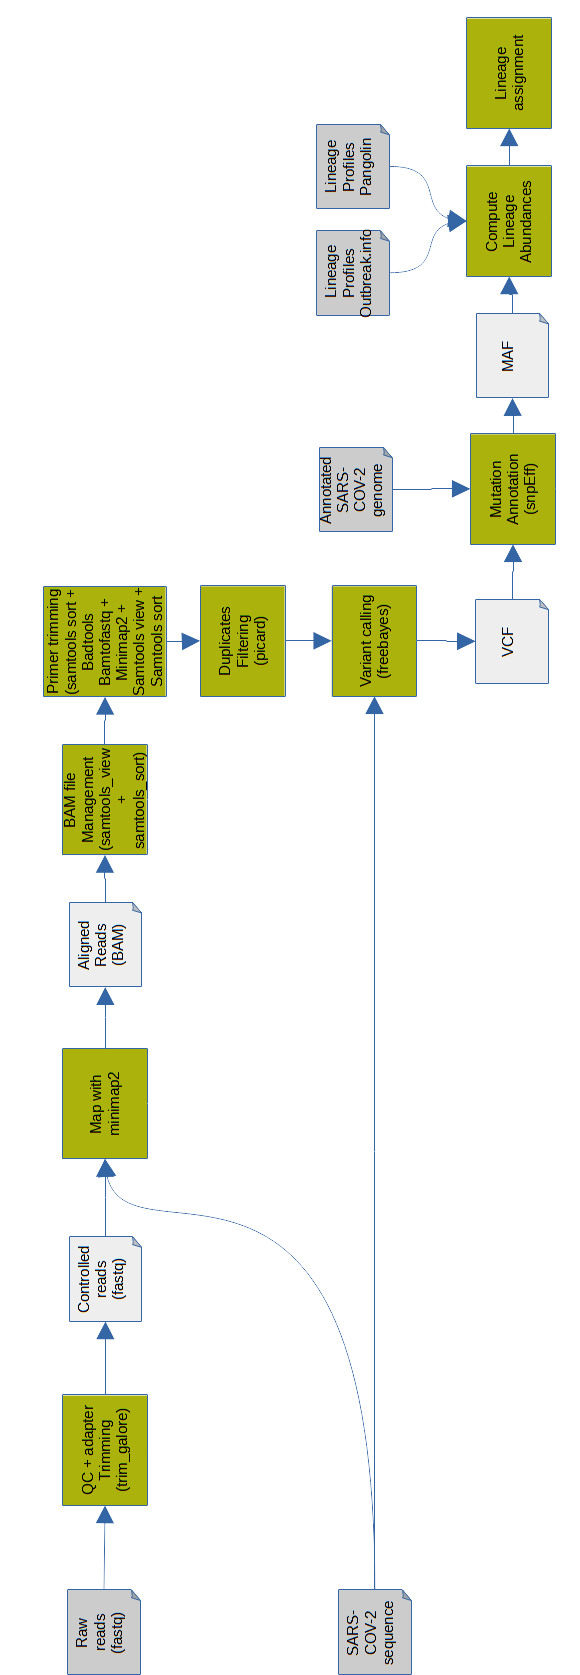
\includegraphics[width=0.5\textwidth]{figures/prior/lineagespot_vertical.png}
            \captionof{figure}{Lineagespot workflow. }
            \label{fig:prior:ls}
        \end{figure}
        
        After computing lineages abundances, Lineagespot provides a set of indicators for each of the provided references. Based on these indicators, the final assignment is made. This additional step in Lineagespot is one of the advantages of this pipeline over others since it allows to mitigate the risk of wrong assigned lineages (e.g. in the case of two groups of reads satisfying different rules for the same lineage but reads from both groups never satisfying all rules for this lineage). According to Lineagespot, several different indicators reflect how many rules are satisfied, how many rules are satisfied based on the detected mutations, and how many reads support each rule both as a reference and as an allele. The drawback of this method is that assignment is made by a semi-automated process but not completely automated.
        
        
        \subsubsection{PiGx}
        The other pipeline, PiGx SARS-CoV-2 \cite{schumann2021}, first, performs extensive quality control on the raw reads and information about primers and adapters used. Fastp \cite{chen2018} is used for adapter trimming and filtering, while iVAR is used for primer trimming. Using BWA \cite{li2013}, the trimmed reads are aligned to the reference genome of SARS-CoV-2, resulting in SAM/BAM files with aligned and unaligned reads. After alignment, MultiQC \cite{multiqc} is used to aggregate reports that check the quality of raw and processed reads. Further, PiGx checks samples for genome coverage and how many of the provided signature mutation sites, sites with mutations that characterize variants of concern or variants of interest, are covered by the sample. Every sample is given a quality score based on this. Those samples with genome coverage of less than 90\% are discarded from time series analyses and summaries.

        With LoFreq \cite{lofreq}, variants are called, and SNVs (single nucleotide polymorphisms) are inferred from aligned reads. The mutations are annotated with VEP \cite{mclaren2016}. 
        
        PiGx is capable of deconvoluting the frequencies of variants of concern from pooled sequencing reads. Briefly, the deconvolution method uses signature mutations for each variant of concern and tries to discern the proportions of these variants making up the observed mutation frequencies in the pooled sequencing reads obtained from the wastewater. To infer the proportions of each lineage on each sample, the deconvolution method is applied (based on the frequencies of the signature mutations). On the basis of the observed frequencies of signature mutations for each lineage, the lineage frequencies are predicted using a regression model. 
        
        After lineage frequencies prediction, PiGx generates a per-sample report that describes variants of concern and frequency of lineages from each wastewater sample. Additionally, the unaligned reads will be taxonomically classified with Kraken2 \cite{wood2014,wood2019,lu2020} to determine the abundance of RNA that matches other existing species found in unaligned reads in the wastewater samples. The diagram of PiGx pipeline is shown in \cref{fig:prior:pigx}.
        
        \begin{figure}[h]
        	\centering
            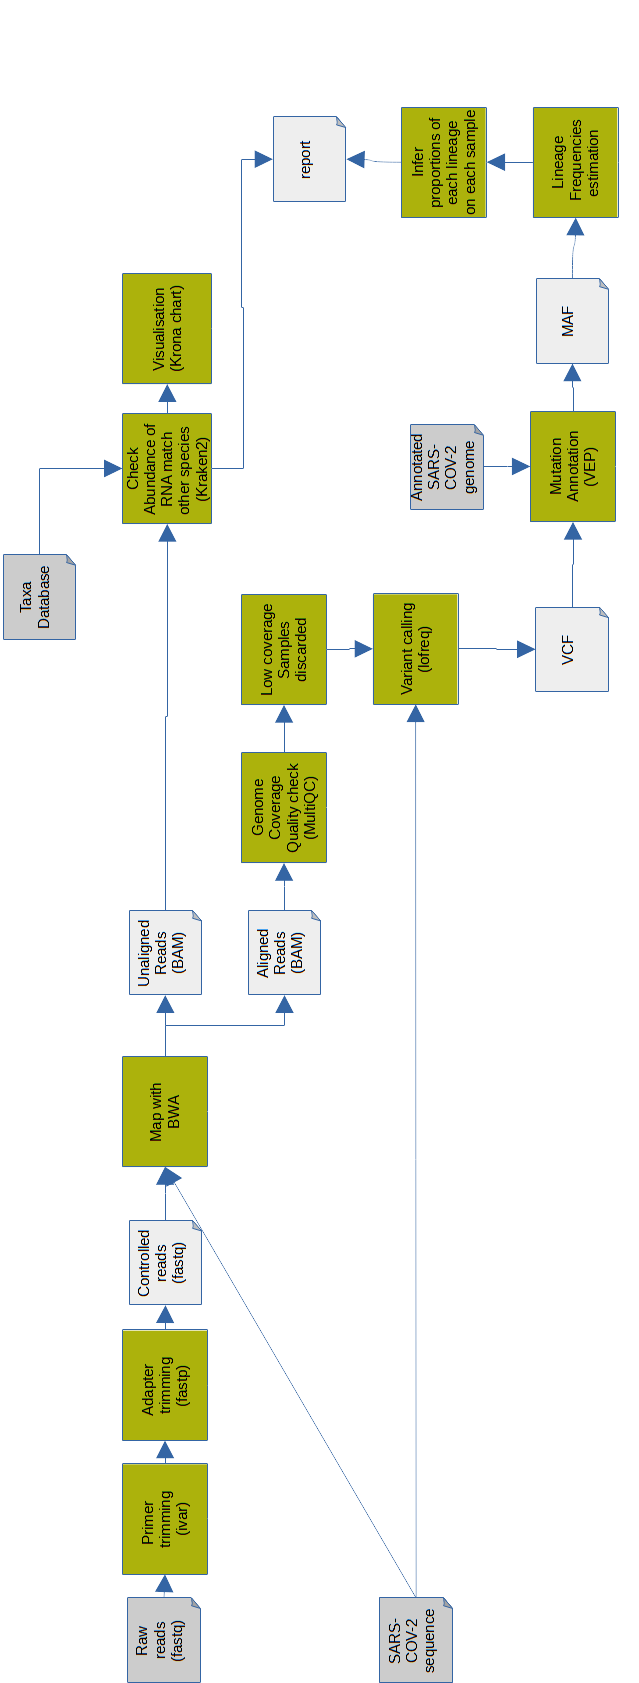
\includegraphics[width=0.5\textwidth]{figures/prior/pigx_vertical.png}
            \captionof{figure}{PiGx workflow. }
            \label{fig:prior:pigx}
        \end{figure}
        
        One of the significant benefits of PiGx method is the addition of different weights of tracked lineages based on how many signature mutations were found for each of them for a given sample. The purpose of this step is to determine which lineages have a low abundance and have only a few or only shared mutations in order to obtain more precise predictions. 

        PiGx has another advantage - controlling taxonomic classification for other species present in samples but not mapped to the SARS-CoV-2 reference sequence. With Kraken2 usage, this simple step opens opportunities for learning about sample diversity. Due to Kraken2's k-mer classification, it can also identify reads that match SARS-CoV-2 but are not aligned with stringent alignment tools. In addition, it provides insights into the possibility of losing new mutations that weren't captured in the alignment. The user can analyze potential issues here and adjust the alignment stringency if necessary.

        \subsubsection{Cowwid}
        In its turn, another approach, Cowwid \cite{jahn2021} pipeline uses steps: 1) processing raw reads with the help of V-pipe \cite{posada2021} sub-workflow (performing quality controls and read filtering with FastQC and PRINSEQ \cite{babraham,prinseq}, assembly with VICUNA \cite{vicuna2012}, read alignment with BWA-MEM and ngshmmalign \cite{li2013,ngshmmalign2021} and variant calling with ShoRAH \cite{shorah}); 2) co-occurrence analysis (detecting mutation co-occurrence) with the help of COJAC \cite{jahn2022,cojac2022}; 3) building of the list of signature mutations for the variants of concern, variant mutation table, and visualization including heatmaps and curves plots generation with the help of Jupyter; 4) generation of Python script for upload to CoV-Spectrum. The diagram that describes the Cowwid workflow is presented in \cref{fig:prior:cowwid}.
        
        \begin{figure}[h]
        	\centering
            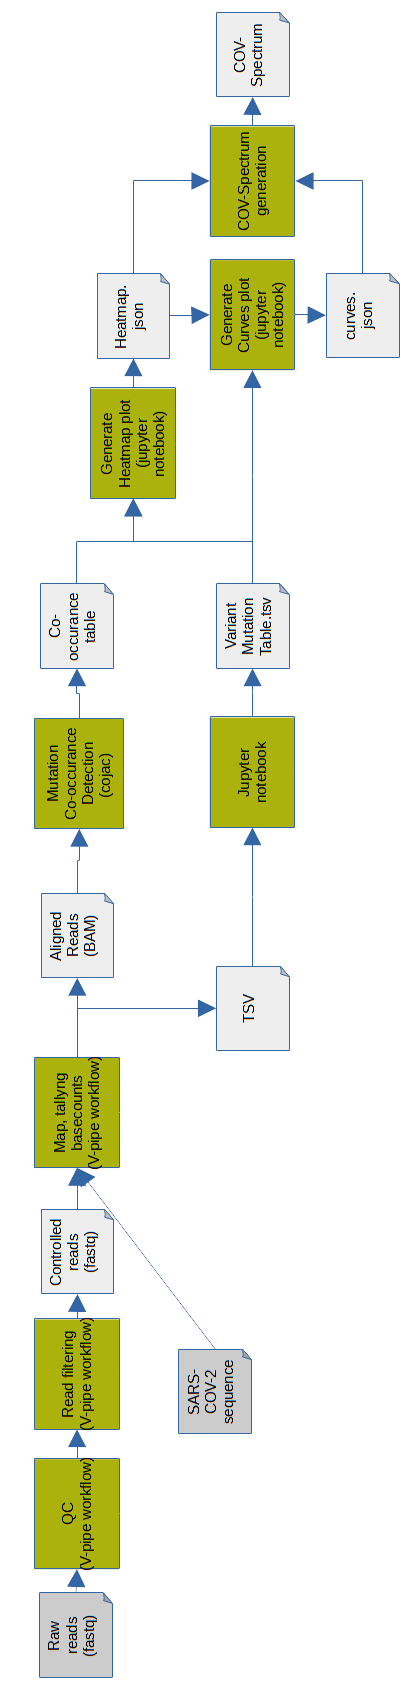
\includegraphics[width=0.3\textwidth]{figures/prior/cowwid_vertical.png}
            \captionof{figure}{Cowwid workflow. }
            \label{fig:prior:cowwid}
        \end{figure}
        
        The advantage of Cowwid pipeline is its capability to detect lineages that are unknown as it uses COJAC tool as a co-occurance step. The other bright side of Cowwid is that its output was already experienced to be uploaded to CoV-Spectrum which means the accessibility of results and a variety of visualizations. Though, the Jupyter-based plots as well as the upload script look hard-coding, which is disadvantageous. That means that this pipeline is advanced but requires to be adjusted and generalized in order to use it for other than datasets described by K. Jahn et al. \cite{jahn2022}. 
        
        \subsubsection{Pipeline described by R. Izquierdo-Lara et al.}
        
        Meanwhile, R. Izquierdo-Lara et al. \cite{izquierdo} used 2 different workflows using two different workflow managers (Snakemake and Galaxy). For the Nanopore data, they used Snakemake to: 1) demultiplex FASTQ raw reads using Porechop \cite{wick2022}; 2) trim of primers using Cutadapt \cite{martin2011}; 3) perform a reference-based alignment against SARS-CoV-2 reference sequence using minimap2; 4) confirm mutations in the genome by manually checking the alignment in UGENE \cite{okonechnikov2012} and resolve homopolymeric regions by consulting reference genomes. On the other hand, for the Illumina Sequence Analysis, they used Galaxy to: 1) filter raw sequencing reads using Fastp \cite{chen2018}; 2) using BWA-MEM, remove adapter contamination, ambiguous bases, low quality reads (Phred score <30), and fragments <50 nt; then, map reads against GISAID sequence EPI\_ISL\_412973; 3) realign reads using FreeBayes \cite{garrison2012}; 4) generate consensus sequences and variants using iVar \cite{grubaugh2019}; 5) finally, confirm variant calling by manual inspection of the aligned reads using UGENE.

        For the phylogenetic analysis, sequences were aligned with >75\% genome coverage using MAFFT \cite{mafft}, followed by visualization of trees with Figtree \cite{figtree}, and clades assignment with Nextclade tool \cite{nextclade2022}. The diagram that describes the workflow is presented in \cref{fig:prior:izquierdo}.
        
        \begin{figure}[h]
        	\centering
            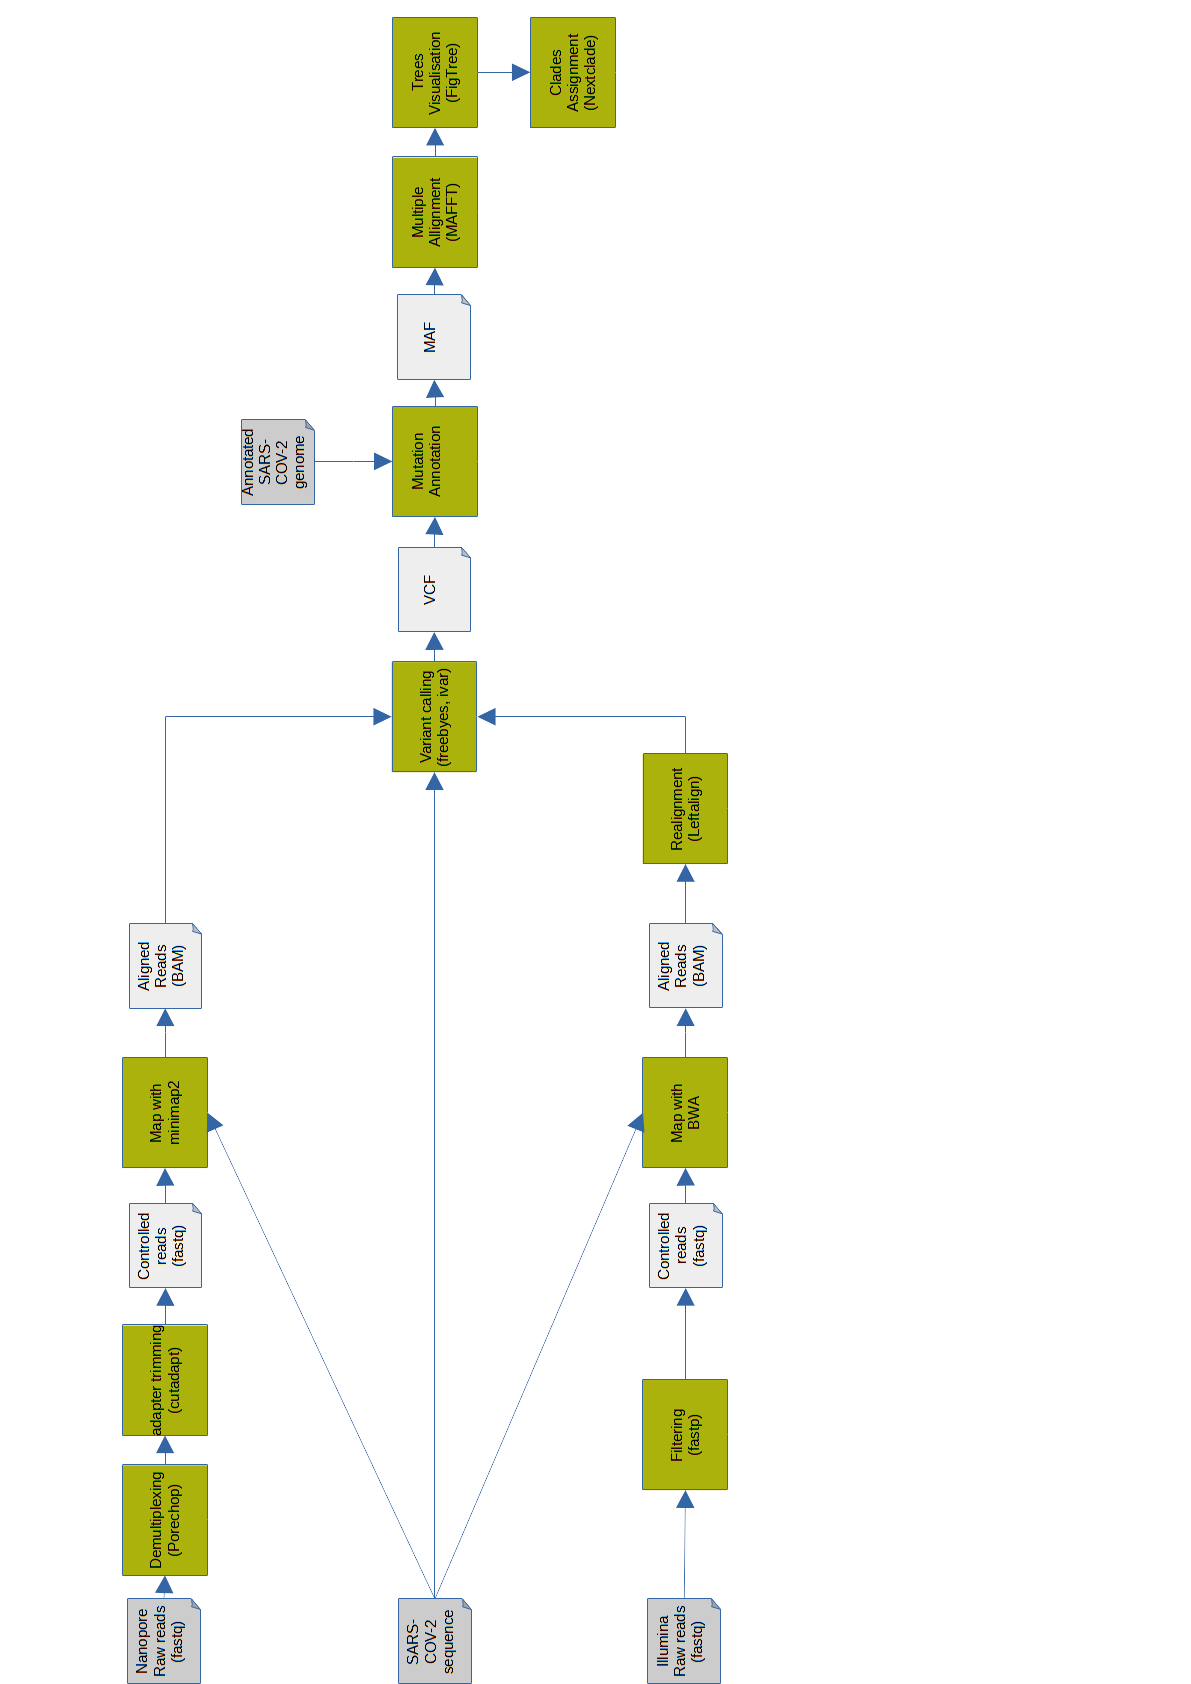
\includegraphics[width=1\textwidth]{figures/prior/Izquierdo-Lara_vertical.png}
            \captionof{figure}{Workflow described by R. Izquierdo-Lara et al.}
            \label{fig:prior:izquierdo}
        \end{figure}
        
        A feature that this pipeline offers that others listed above in this section do not is phylogenetic analysis and visualization of the phylogenetic tree.

    \subsection{Discussion of existing methods} \label{sec:prior:discussion}
    Several methods were described above. These methods use different models to determine SARS-CoV-2 lineages and their abundances in wastewater samples. Several of the methods listed can be applied to the purpose of this thesis, i.g. improvement of existing Galaxy workflows for analyzing SARS-CoV-2 clinical samples, repurposing them to detection of SARS-CoV-2 variants in wastewater samples as well as discerning of lineage abundances in these samples. It should be noted that in section ... (Methods for wastewater surveillance), there are listed not only tools that focus directly on lineage abundance computation, but also complete and almost complete pipelines like PiGx, Lineagespot, Cowwid, etc. that include the entire raw reads bioinformatics analysis. They are not intended to be improved. Conversely, tools that are capable to use the output of existing Galaxy workflows and perform lineage abundances computation are interest of this thesis.

    Two tools, Freyja \cite{joshuailevy2022,karthikeyan2022} and COJAC \cite{jahn2021} were my choices to use in my workflow to achieve the goal of this thesis. Roughly speaking, these tools are different in purpose, for example, Freyja’s output is easy to interpret without some specific knowledge, while COJAC requires more knowledge to be used. First of all, it demands some knowledge in programming as the output of COJAC is quite raw so far and has to be processed for downstream analysis like plotting and integrating to remote platforms such as CoV-Spectrum. Second of all, the usage of COJAC requires some knowledge of virology. In spite of this, COJAC provides more detailed information and is able to detect unknown variants. These two different tools, Freyja and COJAC, target different user groups (e.g. politicians and researchers), which is interesting for the purposes of the research in this thesis.
       
